% Created 2016-09-29 Thu 21:03
\documentclass[11pt]{article}
\usepackage[utf8]{inputenc}
\usepackage[T1]{fontenc}
\usepackage{fixltx2e}
\usepackage{graphicx}
\usepackage{longtable}
\usepackage{float}
\usepackage{wrapfig}
\usepackage{soul}
\usepackage{textcomp}
\usepackage{marvosym}
\usepackage{wasysym}
\usepackage{latexsym}
\usepackage{amssymb}
\usepackage{hyperref}
\tolerance=1000
\providecommand{\alert}[1]{\textbf{#1}}

\title{fast-rcnn}
\author{shhs}
\date{\today}
\hypersetup{
  pdfkeywords={},
  pdfsubject={},
  pdfcreator={Emacs Org-mode version 7.9.3f}}

\begin{document}

\maketitle

\setcounter{tocdepth}{3}
\tableofcontents
\vspace*{1cm}

\section{Fast R-CNN --Ross Girshick}
\label{sec-1}


Paper: \href{http://arxiv.org/abs/1504.08083}{Fast R-CNN}
Code: \href{https://github.com/rbgirshick/fast-rcnn}{Fast R-CNN's code}
\subsection{Fast R-CNN architecture}
\label{sec-1-1}


   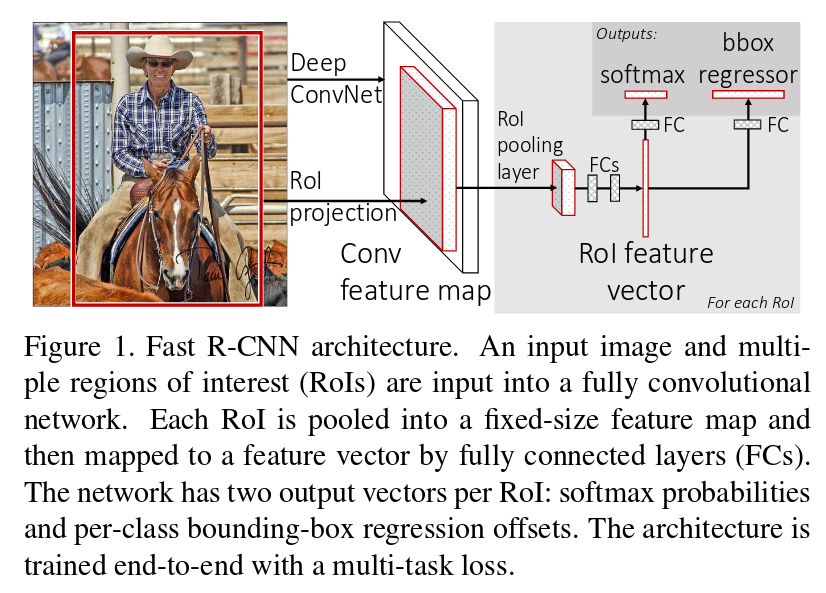
\includegraphics[width=.9\linewidth]{./pic_fast_rcnn/1.png}
\begin{itemize}
\item inputs: \textbf{an entire image}, \textbf{a set of object proposals}
\item several convolutional and max pooling layers -> produce a conv feature map
\item for each object proposal: a RoI(region of interest) pooling layer extracts a 
     fixed-length feature vector from the feature map
\item each feature vector is fed into a sequence of fully connected(fc) layers 
     that finally branch into two sibling(兄弟,姐妹,同属) output layers:
     \textbf{one} that produces softmax probability estimates over K object classes
     plus a catch-all ``background'' class and \textbf{another layer} that outputs 
     four real-valued numbers for each of the K object classes.
\item $\Box$ ? 2. \emph{Each set of 4 values encodes refined bounding-box positions for one of            the K classes.}
\end{itemize}
\subsubsection{The RoI pooling layer}
\label{sec-1-1-1}

\begin{itemize}
\item The RoI pooling layer uses max pooling to convert the features inside any valid
\end{itemize}
    region of interest into a small feature map with a fixed spatial extent of HxW,
    wherer H and W are layer hyper-parameters that are independent of any particular RoI.

\begin{itemize}
\item RoI: (r,c,h,w) specifies its top-left corner(r,c) and its height and width(h,w).
\item RoI max pooling layer divides the hxw RoI window into an HxW grid of sub-windows of
      approximate size h/H x w/W and then max-pooling the values in each sub-window into 
      the corresponding output grid cell.
\end{itemize}
\subsubsection{Initializing from pre-trained networks}
\label{sec-1-1-2}


\begin{itemize}
\item When a pre-trained network initializes a Fast R-CNN network, it undergoes three
      transformations:
\begin{enumerate}
\item The last max pooling layer is replaced by a RoI pooling layer that is configured
         by setting H and W to be compatible with the net's first fully connected layer
         (e.g., H = W = 7 for VGG16).
\item The network's last fully connected layer and softmax are replaced with the two 
         sibling layers described earlier: a fully connected layer and softmax over K + 1
         categories, category-specific bounding-box regressors.
\item The network is modified to take two data inputs: a list of images and a list of
         RoIs in those images.
\end{enumerate}
\end{itemize}
\subsubsection{Fine-tuning for detection}
\label{sec-1-1-3}


\begin{itemize}
\item In Fast R-CNN training, stochastic gradient descent(SGD) mini-batches are sampled 
      hierarchically.
\begin{enumerate}
\item First sampling N images
\item Second sampling R/N RoIs from each image.
\end{enumerate}
\item RoIs from the same image share computation and memory in the forward and backward
      passes.
\item One concern over this strategy is it may cause slow training convergence because
      RoIs from the same image are correlated. This concern does not appear to be a 
      practical issue and we achieve good results with N = 2 and R = 128 using fewer
      SGD iterations than R-CNN.
\end{itemize}
\begin{itemize}

\item Multi-task loss\\
\label{sec-1-1-3-1}%
\begin{itemize}
\item A Fast R-CNN network has two sibling output layers.
\begin{enumerate}
\item The first outputs a discrete probability distribution(per RoI), 
          $p = (p_0, ..., p_K)$, over K + 1 categories.(a softmax over the K + 1 outputs of a
          fully connected layer.
\item The second sibling layer outputs bounding-box regression offsets, 
          $t^k = (t_x^k, t_y^k, t_w^k, t_h^k)$, for each of the K object classes, indexed by k.
\item $\Box$ We use the parameterization for $t^k$ given in \footnote{R. Girshick, J. Donahue, T. Darrell, and J. Malik.  
  Rich feature hierarchies for accurate object detection and semantic segmentation. In CVPR, 2014.
 }, in which t$^k$ specifies a
          scale-invariant translation and log-space height/width shift relative to an object 
          proposal.
\end{enumerate}
\item Each trainging RoI is labeled with a ground-truth class u and a ground-truth bounding-box
       regression target v. We use a multi-task loss L on each labeled RoI to jointly train for
       classification and bounding-box regression:
       \begin{equation}
       L(p, u, t^u, v) = L_{cls}(p, u) + \lambda[u\ge1]L_{loc}(t^u, v)         
       \end{equation}
       in which $L_{cls}(p, u)  = -logp_u$ is log loss for true class u.
\item The second task loss , $L_loc$, is defined over a tuple of true bounding-box regression 
       targets for class u. The Iverson bracket indicator function $[u\ge1]$ evaluates to 1 when 
       $u>1$ and 0 otherwise.For background RoIs there is no notion of a ground-truth bounding box
       and hence $L_{loc}$ is ignored. For bounding-box regression, we use the loss
       \begin{equation}
         L_{loc}(t^u, v) = \sum_{i\in{x, y, w, h}} smooth_{L_1}(t_i^u - v_i)         
       \end{equation}
\end{itemize}
       

       in which 
       \$\$smooth$_{\mathrm{L_1}}$(x) = 


       

\end{itemize} % ends low level

\end{document}
